\documentclass[12pt]{article}

\usepackage[french]{babel}
\usepackage[T1]{fontenc}
\usepackage{ragged2e}
\usepackage{amsfonts}
\usepackage{systeme}
\usepackage{amsmath}
\usepackage{amssymb}
\usepackage[top=3cm, bottom=3cm, left=2.5cm, right=2.5cm]{geometry}
\usepackage{comment}
\usepackage{multicol}
\usepackage{lipsum} 
\usepackage{graphicx}
\usepackage{stmaryrd}
\usepackage{systeme}
\usepackage{wrapfig}
\usepackage{colortbl}
\usepackage{cellspace}
\usepackage{stmaryrd}
\usepackage{ntheorem}
\usepackage{lmodern}
\usepackage{mathtools}
\usepackage{ragged2e}
\usepackage{tabularx}
\usepackage{titlepic}
\usepackage{fancyhdr}
\usepackage[hypcap=true]{caption}
\usepackage{xcolor} % pour les couleurs
\usepackage[linkbordercolor=white]{hyperref} % après avoir chargé xcolor
\usepackage{systeme}
\usepackage[T1]{fontenc}
\usepackage{lmodern}
\usepackage{listings}
\usepackage{tikz}
\usepackage{mdframed}
\usepackage{xparse} % Nécessaire pour définir des environnements avec arguments optionnels
\usepackage{booktabs}  % Pour des tableaux plus jolis
\usepackage{tocloft}
\usepackage{pdfpages}
\usepackage{helvet}
\renewcommand{\familydefault}{\sfdefault}
\usepackage{setspace}



% PAGE SETTINGS

\newcolumntype{C}{>{$\displaystyle}Sc<$}
\cellspacetoplimit=5pt
\cellspacebottomlimit=5pt


% OTHERS 

% \newlength\tindent
% \setlength{\tindent}{\parindent}
% \setlength{\parindent}{0pt}
% \renewcommand{\indent}{\hspace*{\tindent}}


\usepackage{fancyvrb}
\usepackage{tikz-cd} 
\usepackage{amsmath}
\usepackage{mathrsfs}  
\usepackage{amssymb}
\usepackage{tkz-graph}
\usepackage{caption}
\usepackage{multicol}
\usepackage{listings} % Importation du package listings
\usepackage{xcolor} % Pour ajouter de la couleur

\setlength{\columnsep}{1cm} % Espace entre les colonnes


% Définition du style de l'en-tête
% \pagestyle{fancy}
\fancyhf{} % Nettoyer les en-têtes et pieds de page
\fancyfoot[C]{\thepage} % numéro de page centré en bas
\pagenumbering{arabic} % numérotation en chiffres arabes (1, 2, 3...)

% Gauche : Nom de la section
% \fancyhead[L]{\nouppercase{\leftmark}}

% Droite : Logo
% \fancyhead[R]{
\includegraphics[width=1cm]{./images/logo_jfc.png}}

% Ligne sous l'en-tête
% \renewcommand{\headrulewidth}{0.4pt}

\onehalfspacing


\begin{document}

% ==================================================================================================================================
% TITLEPAGE 

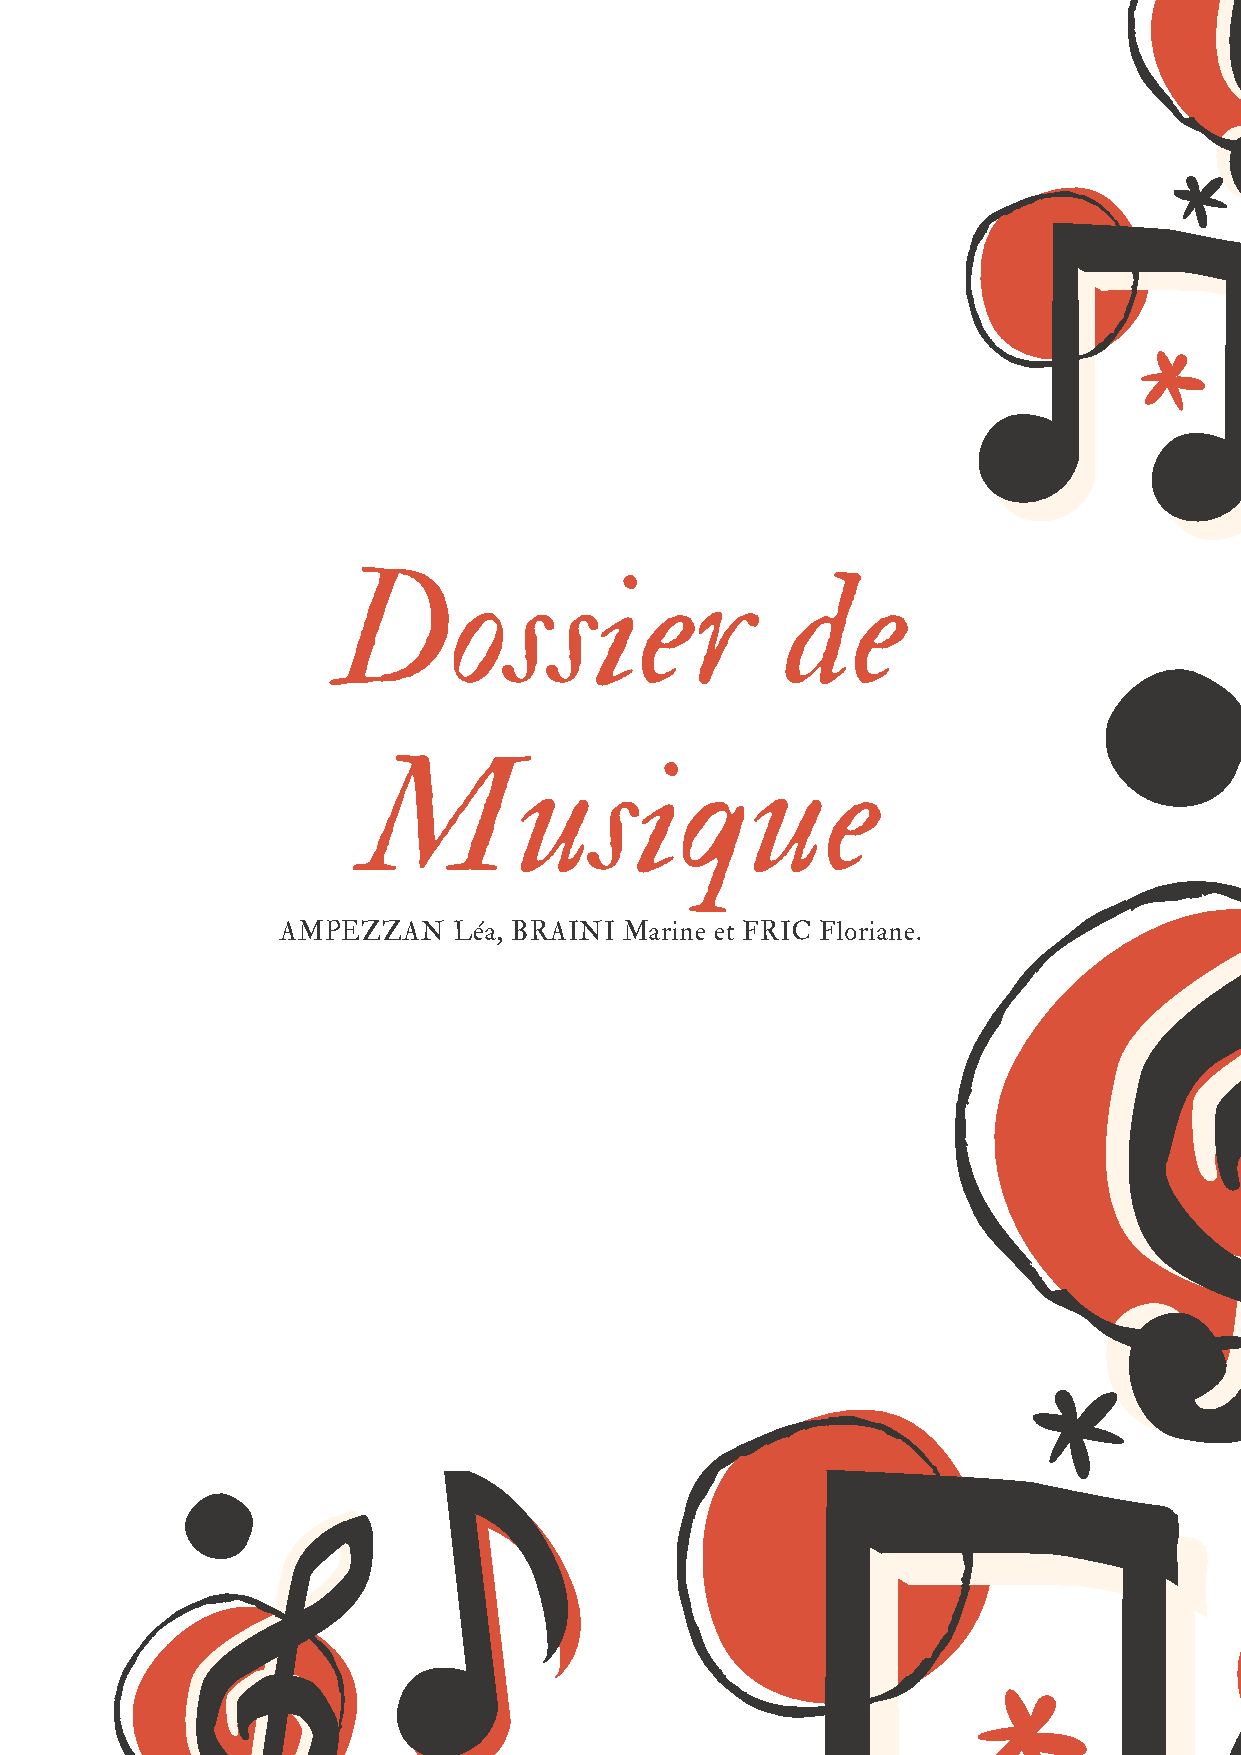
\includepdf[pages=1]{./images/titlepage.pdf}

% ==================================================================================================================================
% ETUDE de l'Oeuvre 

\section{Étude de l'Oeuvre}

Cet extrait musical est un extrait des Quatre saisons d’Antonio VIVALDI, composé entre 1723 et 1725. 
Plus précisément c’est le concerto pour violon op. 8 n°4, « L’hiver » 1er mouvement. 

Antonio VIVALDI était prêtre-maestro. Dès son plus jeune âge, son père lui transmet sa passion pour le violon. 
Il consacre sa vie à la religion catholique ainsi qu’à la musique. D’où le choix de cet instrument, 
pour son aspect lyrique. Au-delà de l'intérêt qu'apporte VIVALDI au violon, il était doté de grandes capacités. 
Il était précoce et doué. Il profita de sa place en tant que maître-violon au sein d’un orphelinat pour composer ses œuvres.
Elles sont diffusées en manuscrit. Antonio VIVALDI est en pleine liberté créative. 
Néanmoins, son esprit d’indépendance lui a valu à plusieurs reprises un vote défavorable par des administrateurs. 
Cependant l’artiste tient tête et devient compositeur de musique. Il est connu pour être l’initiateur du concerto de soliste, 
un genre dérivé du concerto grosso. En effet, il fait la liaison entre deux courants artistiques : baroque et classicisme. 
Le style baroque est enrichi par la basse en continu ainsi que le contraste entre les effets sonores. 
Celui-ci vise à faire ressortir des émotions, à captiver l’attention ou bien à impressionner. 
On y retrouve de grands artistes tels que Jean-Sébastien Bach, Marc-Antoine Charpentier, Jean-Philippe Rameau ou 
bien Domenico Scarlatti. En ce qui concerne le classicisme, la basse disparaît, les structures musicales sont ordonnées. 

Pour finir, Antonio VIVALDI était fortement apprécié par tous et son œuvre "Les Quatre Saisons" est classé parmi les 
plus populaire du répertoire classique. Son histoire est importante car elle marque la transition dans la création artistique de l’époque.

\vspace{0.3cm}

Passons maintenant à l’étude de l’extrait.
Dans cet extrait, nous n’entendons que des instruments à cordes : des violons, des violons alto, des violoncelles, des contrebasses. De plus, nous remarquons un clavecin. Nous distinguons très rapidement deux groupes : une violoniste soliste d’un côté et de l’autre l’orchestre formé de tous les autres instruments. Pour étudier plus précisément cet extrait nous avons décidé de le découper en trois parties.

La \textbf{première partie} se construit petit à petit avec l’addition successive des instruments. Le clavecin commence puis est suivi par les cordes. Enfin la soliste apparaît. Tous jouent des notes saccadées à différentes hauteurs, les contrebasses et les violoncelles étant les plus graves et la soliste la plus aiguë. Cela créer une sensation de tension et de stress. Ils sont en train de mettre en place un ostinato. 
Subitement, la soliste se différencie du reste de l'orchestre en jouant des notes beaucoup plus rapides et plus aiguës. Pendant les apparitions du soliste, l’orchestre s’arrête de jouer. Un question-réponse se met en place entre la soliste qui fait des envolées et les autres musiciens qui gardent l’ostinato et où chacun des groupes arrête de jouer lorsque l’autre joue. Lors du troisième échange, la soliste se fond à nouveau dans l’orchestre comme au début. Ainsi, cela fait augmenter la nuance et vient renforcer la montée en puissance du morceau menant à la deuxième partie de cette œuvre.

Au cours de la \textbf{deuxième partie}, tous les instruments jouent en même temps la même mélodie. Or nous arrivons à distinguer les deux plans sonores entre la soliste et l’orchestre. On perd ainsi l’ostinato et donc le sentiment d’angoisse qu’il procurait. On a l’impression que le morceau a accéléré et un sentiment de course poursuite s’installe. Puis, tous les instruments s’arrêtent de jouer sauf la soliste, le clavecin et les violoncelles. Ce moment nous donne l’impression d’avoir un moment de répit, qui n’est malheureusement que de courte durée car rapidement tous les autres musiciens reviennent. Un léger question-réponse revient entre la soliste et l’orchestre mais cette fois-ci l’orchestre vient amplifier certains passages du soliste.

On arrive directement dans la \textbf{troisième partie} du morceau qui est un mélange des deux premières parties. En effet, l’ostinato et le thème de la soliste de la première partie reviennent. Puis ils laissent leur place au thème de la deuxième partie pour finir le morceau tous ensemble.

Ce morceau est bel et bien un concerto car on y retrouve trois mouvements avec différents temps notamment accompagnés d’un échange entre un soliste et l’orchestre.


% ==================================================================================================================================
% ACTIVITES

\section{Propositions de séances}

À travers la \textbf{première séance}, les élèves découvrent L’Hiver de Vivaldi à travers une approche originale mêlant écoute active, expression orale et création narrative. L’objectif est de les amener à imaginer une histoire inspirée par la musique, puis à la raconter à voix haute. Cette activité stimule à la fois l’imaginaire, la sensibilité artistique, et les compétences langagières. 
La séance débute par une écoute attentive de l’extrait L’Hiver. Les élèves expriment librement ce que la musique leur évoque. Ensuite, par petits groupes, les élèves imaginent une courte histoire en lien avec la musique. Celle-ci doit suivre une structure simple comprenant un début, un problème, une résolution et une fin. L’enseignant peut accompagner dans la rédaction. Une fiche-guide pourrait les aider. Chaque groupe rédige son texte. Pour ceux qui ont de l’avance, ils peuvent commencer à se le partager et à le répéter à voix haute, en travaillant l’intonation, l’articulation. L’objectif est que leur narration soit fluide et expressive. Par la suite, les élèves passent par groupes devant le reste de la classe pour exprimer leur histoire. On finit sur un moment d’échange, de valorisation et d’appréciation du travail de chacun, l’échange final permettra d’institutionnaliser la séance. L’objectif est de permettre aux élèves de développer leur écoute musicale, leur expression orale, leur créativité et leur coopération. Elle sensibilise la musique classique et la rend vivante en montrant que l’on peut l’écouter autrement en inventant ses propres histoires. Pour finir, on institutionnalise la séance.

Au cours de la \textbf{deuxième séance}, nous rappelons le déroulement de la séance précédente ainsi que la mise en commun. Nous faisons une écoute de l’œuvre en prenant seulement les 40 premières secondes environ. Dans un premier temps, la classe est divisée en deux pour chercher des idées de sons possibles à produire à l’aide de son corps (souffler, frapper, frotter,etc). Par la suite, les élèves présentent à l’ensemble de la classe les sons qu’ils ont pu trouver. Désormais, les élèves se mettent par petits groupes et ils vont devoir essayer de reproduire l’orchestre entendu grâce aux sons trouvés auparavant. Une fois trouvés et organisés, ils présenteront leur création devant l’ensemble de la classe. Pour finir, on institutionnalise la séance.

Pour la \textbf{troisième séance}, nous ferons une écoute de la deuxième partie de l’œuvre. C'est-à-dire le moment question-réponse entre la soliste et le chœur. 
Par petits groupes, les élèves cette fois-ci vont devoir se mettre en accord sur un codage autour de la partie du soliste ainsi que celle sur l’orchestre. Après environ 15 minutes, on finit par un moment d’échange sur les différents codages et les élèves justifient leurs choix. Une fois l’échange finit, l’ensemble de la classe écoute le reste de l’extrait. Un débat est organisé pour relever les similitudes entre la fin du passage ainsi que le commencement. Il est possible pour l’enseignant de faire écouter une autre « saison » de VIVALDI pour repérer les liens entre les extraits et amenés l’esprit des différentes saisons. Pour finir, on institutionnalise la séance.

% ==================================================================================================================================
% CONCLUSION

\section{Conclusion}

À travers l’étude de l’œuvre L’Hiver d’Antonio Vivaldi, ce dossier a permis de mettre en lumière la richesse expressive de la musique baroque ainsi que l’ingéniosité de son compositeur. L’analyse de l’extrait, tant sur le plan musical que pédagogique, a révélé l’intérêt de cette œuvre pour développer l’écoute active, l’expression orale, l’imagination et la créativité des élèves.
Les séances proposées montrent que la musique classique peut être un puissant vecteur d’apprentissage, de coopération et de plaisir partagé. En intégrant des approches sensorielles, corporelles et narratives, les élèves sont amenés à s’approprier une œuvre du répertoire tout en développant des compétences transversales.
Ce travail met ainsi en avant l’importance de faire vivre la musique à l’école de manière vivante, ludique et signifiante, en la plaçant au cœur d’un projet artistique et pédagogique global.


\end{document}
